\documentclass[12pt]{article}

\usepackage[letterpaper, margin=1in]{geometry}
\usepackage{amsmath}
\usepackage{enumerate, subcaption, graphicx, hyperref, hhline}
\usepackage{adjustbox}
\usepackage{array} 
\usepackage[utf8]{inputenc}
\usepackage{listings}
\usepackage{xcolor}

\begin{document}


\section{Introduction}

Homelessness remains one of the most pressing issues around the world. It is a complex issue influenced by a myriad of economic and social factors which makes it a challenging problem to address. As such, understanding the dynamics that lead to homelessness is crucial for developing effective interventions and policies. This research project seeks to explore the factors contributing to homelessness rates in the United States using regression analysis. 

\section{Dataset Description}

To address this problem, we used the dataset \cite{nisar_2019_market} collected by a research group affiliated with the Department of Housing and Urban Development. This dataset encompasses the Point-in-Time count of homeless people with a wide array of socioeconomic, demographic, environmental, and policy-related variables. The statistical units are Continuum of Care (CoC) areas in the United States, which are regional planning bodies that coordinate housing and services funding for homeless people. The CoC areas are organized in various ways, and each CoC may cover a specific city, metropolitan area, or multiple counties.

For this study, we have taken a subset of the original dataset to only include variables we are interested in from the year 2017, which contains the least amount of missing values. Table~\ref{tab:variables} lists the variables we used.

\begin{table}[htp]
    \centering
    \begin{adjustbox}{max width=\textwidth}
    \Large
    \begin{tabular}{lcc}
        \hline
        \textbf{Name} & \textbf{Description} & \textbf{Type} \\
        \hline
        pit\_hless\_pit\_hud\_share & Number of homeless people per 10,000 population & Numeric \\
        hou\_mkt\_medrent\_acs5yr\_2017 & Median rent & Numeric \\
        hou\_mkt\_homeval\_acs5yr\_2017 & Median housing unit value & Numeric \\
        
        urban\_cat & Urbanicity with 1: rural, 2: suburban, 3: urban, 4: large city & Categorical \\
        
        econ\_labor\_medinc\_acs5yr\_2017 & Median Income & Numeric \\
        
        econ\_labor\_unemp\_rate\_BLS & Unemployment rate & Numeric \\
        
        econ\_labor\_incineq\_acs5yr\_2017 & Gini coefficient 2016 & Numeric \\
        
        hou\_mkt\_homeage1940\_acs5yr\_2017 & Percentage of housing units built before 1940 & Numeric \\
        
        hou\_pol\_occhudunit\_psh\_hud & HUD unit occupancy rate & Numeric \\
        
        dem\_soc\_ed\_lesshs\_acs5yr\_2017 & Share of the population without high school diploma & Numeric \\
        
        dem\_soc\_hispanic\_census\_share & Share of Hispanic Population & Numeric \\
        
        dem\_pop\_mig\_census\_share & Yearly Increase in Population to Total Population & Numeric \\
        
        env\_wea\_avgtemp\_noaa & Average January Temperature & Numeric \\
        
        env\_wea\_precip\_annual\_noaa & Total Annual Precipitation & Numeric \\
        \hline
    \end{tabular}
    \end{adjustbox}
    \caption{Variable Descriptions}
    \label{tab:variables}
\end{table}



\section{Research Questions}

Going into this research project we have three main questions that we want to answer:
\begin{enumerate}
    \item Can we use a linear model to fit the relationship between the homeless rate and the data?
    
    \item Which factors appear to affect the homelessness rate most significantly?

    \item Do the significant variables in our model change depending on the region in which the data is collected?
    
\end{enumerate}


\section{Methodology}

In order to answer the questions posed above we created a simple linear model for the homeless rate that included all of the other independent variables. Then, we addressed potential problems and refined the model accordingly. Finally, we removed insignificant variables from the model and used the model to determine if there are significant differences based on region.


\subsection{Linear Regression}

We created a model of the following form:

$Y = \beta_{0} + \beta_{1}X_1 + \beta_{2}X_2 + ... + \beta_{13}X_{13} + \epsilon$


\begin{itemize}
    \item $Y = [y_1, y_2, ..., y_n]$ the vector of observations for the homeless rate

    \item $X_i = [x_1, x_2, ..., x_n]$ the vector of observations for the ith independent variable

    \item $\beta_i$ the regression coefficient for the ith independent variable

    \item $\epsilon$ the vector of error terms such that $\epsilon \sim \mathcal{N}(0, \sigma^2I_n$) with $I_n$ the $n\times n$ identity matrix.

\end{itemize}

We then find the values $\hat{\beta}$ that minimize the residual sum of squares $RSS = (Y-X\beta)'(Y-X\beta)$ for X the design matrix and $\beta$ the vector of regression coefficients for each independent variable. For this project, we used R to do multiple linear regression on our 13 predictor variables.

\subsection{Backward Selection\cite{james_2023_an}}

We used back selection to select the most significant predictors for the model. In this project we did back selection with the following algorithm:
\begin{enumerate}
    \item Create a list of the 13 predictors
    \item For each predictor in the list, create a model which excludes that predictor
    \item Remove the predictor from the list corresponding to the model with the smallest MSE.
    \item Repeat steps 2 and 3 until we have 5 predictors left.
\end{enumerate}
This results in a model with predictors such that it has the lowest possible error.


\section{Results}
\subsection{Linear Regression Model Construction}

\subsubsection{Model with all the variables}
We first fitted a model to predict the homeless rate with all the variables without transformation or regularization. Figure~\ref{subfig:simple} shows the distribution of the residuals. Notice that there are non-linear patterns in the residual-fitted plot and the variance of residuals is not constant. One potential reason is the outliers and high-leverage samples identified in the residual-leverage plot, which interfered with the regression.

\begin{figure}[htp]
    \centering
    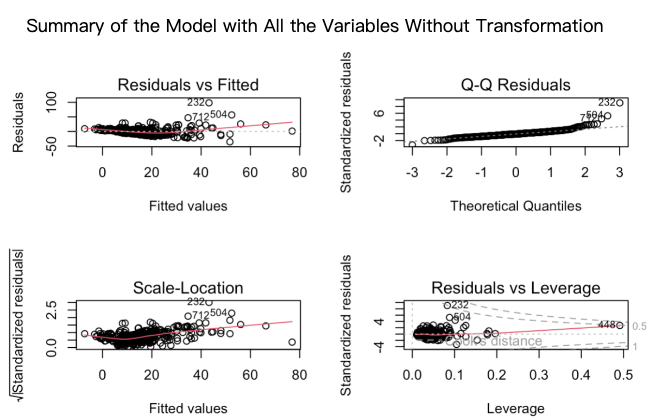
\includegraphics[width = 0.6\textwidth]{simple.png}
    \caption{Analysis of the residuals generated by the models with all the variables and without transformation or regularization}
    \label{fig:simple}
\end{figure}

Therefore, we analyzed these influential points and tried to remove them to improve the model's performance. To identify the influential points, we calculated Cook's distance and the leverage for each sample. We took the conventional thresholds of $4/N$ for Cook's distance and $2\mu$ for the leverage, where $N$ denotes the number of samples and $\mu$ denotes the mean leverage. There are 22 samples exceeding the threshold of Cook's distance, 25 samples exceeding the leverage threshold, and in total 35 samples. 

We hypothesized that these influential points may come from megacities like San Fransico with distinct contexts, so we analyzed the urbanicity of these samples. Figure~\ref{subfig:outlier_urban} compares the proportions of different urbanicity categories among the influential points and all the samples. There is no significant difference between the distributions, and there are many samples from rural or suburban areas among the outliers and the high-leverage points. 

What distinguishes them from the other samples is the high homeless rate. Figure~\ref{subfig:outlier_pit} shows that the distribution of the homeless rate among all the samples is right-skewed with a low average value. The outliers and the high-leverage points on average have a higher homeless rate, coming from the tail of the skewed data. Given the skewness of the response's distribution, we decided to apply the logarithm transformation to the response to make its distribution more symmetric and help normalize the residuals, instead of dropping the influential points.

\begin{figure}[htp]
    \centering
    \begin{subfigure}[b]{.45\textwidth}
    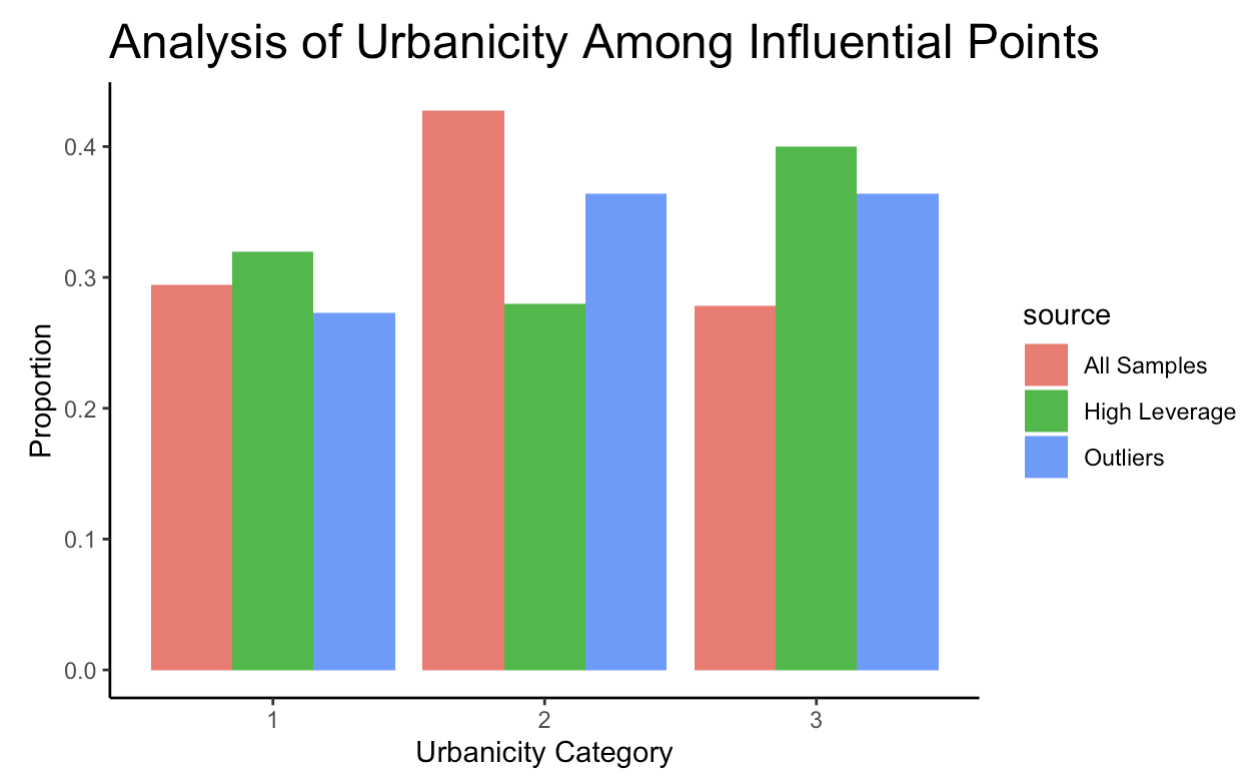
\includegraphics[width=\textwidth]{outlier_urban.png}
    \caption{}
    \label{subfig:outlier_urban}
    \end{subfigure}
    \begin{subfigure}[b]{.45\textwidth}
    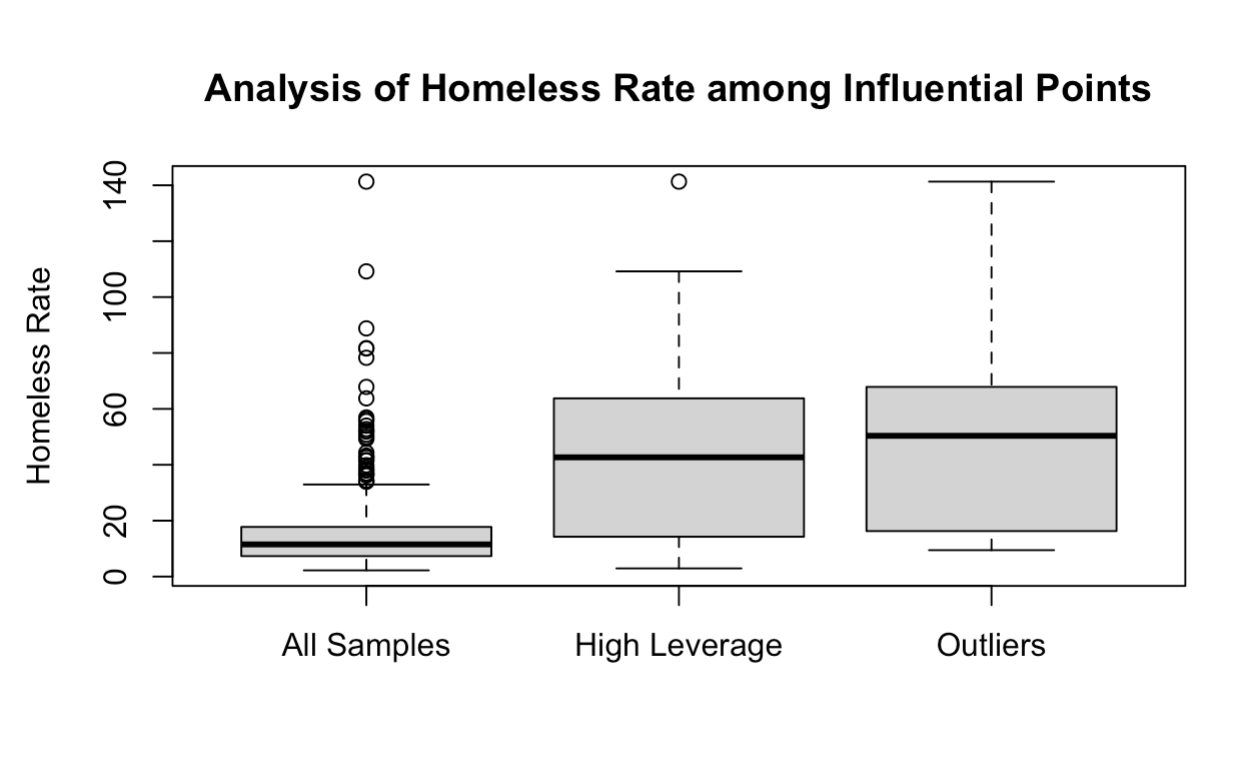
\includegraphics[width=\textwidth]{outlier_pit.png}
    \caption{}
    \label{subfig:outlier_pit}
    \end{subfigure}
    \caption{Comparison between the identified influential points and all the samples}
    \label{fig:outliers}
\end{figure}

\subsubsection{Model with all the variables and log-transformation}

We applied the logarithm transformation to the homeless rate and refitted the regression again with all the variables. Figure~\ref{fig:log} shows the distribution of the residuals generated by the model. This time the residuals are distributed normally with a good fit to the line on the Q-Q plot. The residuals also have a constant variance on the scale-location plot. The model has a reasonable performance with $R^2 = 0.4917$ in predicting such a complex social problem. However, the linear regression model also has assumptions about the linear independence of predictors and the independence of errors that we need to check. 

\begin{figure}[htp]
    \centering
    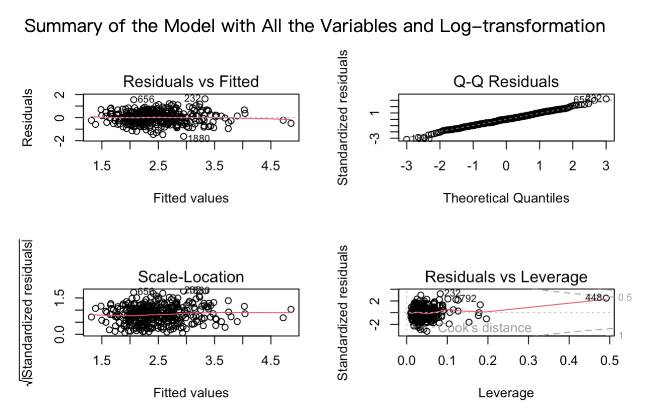
\includegraphics[width = 0.6\textwidth]{log.png}
    \caption{Analysis of the residuals generated by the models with all the variables and log-transformation to the response.}
    \label{fig:log}
\end{figure}

We performed a Durbin-Watson test to detect the autocorrelation between errors. The null hypothesis is that there is no autocorrelation, and the alternative is that the autocorrelation does not equal 0. In this setting, we got the Durbin-Watson statistic = 1.6781 and p-value = 0.0007846, indicating that there is a significant autocorrelation between errors.

Meanwhile, we used the Variance Inflation Factor (VIF) to measure the collinearity between predictors. Since we have a categorical variable that has been transformed into dummy variables, we calculated the adjusted Generalized Variance Inflation Factor (GVIF) instead. Table~\ref{tab:gvif} lists the results. Variables \texttt{econ\_labor\_medinc\_acs5yr}, \texttt{hou\_mkt\_medrent\_acs5yr}, and \texttt{hou\_mkt\_homeval\_acs5yr} that refer to the median income, the median rent, and the home value have relatively high values. Indeed, they are all related to the economic level of the area and correlate with each other and other variables.

The autocorrelation between errors and the collinearity between predictors violate the assumptions of linear regression, leading to less precise estimates. We addressed these problems by introducing new variables and transforming the existing variables.

\begin{table}[htp]
\centering
\begin{tabular}{lcc}
\hline
\textbf{Variable} & \textbf{GVIF} & \textbf{GVIF\^{}1/(2*Df)} \\
\hline
dem\_soc\_ed\_lesshs\_acs5yr & 3.583773 & 1.893086 \\
econ\_labor\_incineq\_acs5yr & 1.890769 & 1.375052 \\
econ\_labor\_medinc\_acs5yr & 7.499974 & 2.738608 \\
hou\_mkt\_homeval\_acs5yr & 8.380482 & 2.894906 \\
hou\_mkt\_homeage1940\_acs5yr & 1.952499 & 1.397319 \\
hou\_mkt\_medrent\_acs5yr & 15.023240 & 3.875982 \\
econ\_labor\_unemp\_rate\_BLS & 1.774055 & 1.331937 \\
hou\_pol\_occhudunit\_psh\_hud & 1.073627 & 1.036160 \\
env\_wea\_precip\_annual\_noaa & 1.543465 & 1.242363 \\
env\_wea\_avgtemp\_noaa & 2.762188 & 1.661983 \\
dem\_pop\_mig\_census\_share & 1.621306 & 1.273305 \\
dem\_soc\_hispanic\_census\_share & 3.575583 & 1.890921 \\
urban\_cat & 1.977822 & 1.185897 \\
\hline
\end{tabular}
\caption{GVIF values calculated for the model with all the variables and log-transformation}
\label{tab:gvif}
\end{table}

\subsubsection{Model with Region and log-transformation}

We hypothesized that the autocorrelation between errors comes from the spatial relation between the samples. The CoC areas in the same state or the same region are in similar contexts (e.g. policy, history, and culture), and the homeless rates in these areas might be correlated. Therefore, we introduced a new variable \texttt{Region} to capture this spatial relation and explain the residuals.

\texttt{region} is a categorical variable and records the statistical regions (Northeast, Midwest, South, and West) that the CoC areas are located at. It is defined by the US Census Bureau and organized in the dataset\cite{halpert_2023_cphalpertcensusregions}. With this new variable, our model had a better performance with $R^2 = 0.5295$. The Durbin-Watson test gave that DW = 1.85 and p-value = 0.07711, indicating that the autocorrelation reduces.

\subsubsection{Model with Region, inc\_val\_rate and log-transformation}\label{sec:final_model}

The median income, the median rent, and the median house value in an area are highly correlated with each other. We did not want to remove any of them and lose information about the homeless rate, so we decided to create a composite variable by combining them.

We created a variable called \texttt{inc\_val\_rate} that is computed by dividing the median house value by the median income. It combines the information of these two variables and measures their relationship. \texttt{inc\_val\_rate} is also interpretable and can be understood as the time it takes for a median person to buy a median house. The model that replaced the median income and the median house value with this composite variable had $R^2 = 0.5193$ and GVIF values listed in Table~\ref{tab:gvif_final}. All the GVIF values decreased, indicating less collinearity.

\begin{table}[ht]
\centering
\begin{tabular}{lcc}
\hline
\textbf{Variable} & \textbf{GVIF} & \textbf{GVIF\^{} 1/(2*Df)} \\
\hline
hou\_mkt\_medrent\_acs5yr & 4.612244 & 2.147614 \\
inc\_val\_rate & 3.784229 & 1.945309 \\
\hline
\end{tabular}
\caption{GVIF values calculated for the median rent and the new variable \texttt{inc\_val\_rate}}
\label{tab:gvif_final}
\end{table}

In this model, we used the new variable \texttt{region} and replaced the median income and the median house value with their ratio \texttt{inc\_val\_rate} to predict the log-transformed homeless rate. We took this linear regression model as our baseline for further exploration.

\subsection{Significant Variable Selection}\label{sec:significant}

We performed a backward selection on the linear regression model we constructed in Section~\ref{sec:final_model}. It revealed the most significant five variables that affect the homeless rate in an area. Table~\ref{table:regression-output} summarized the results. The percentage of houses built before 1940, the median rent, the urbanicity, the region, and the ratio between income and house value turned out to be the most significant. 

\begin{table}[ht]
\centering
\begin{tabular}{lcccc}
\hline
\textbf{Variable} & \textbf{Estimate} & \textbf{Std. Error} & \textbf{t value} & \textbf{Pr}$\mathbf{(>|t|)}$ \\
\hline
(Intercept) & 1.4912 & 0.1120 & 13.319 & $<$ 2e-16 *** \\
hou\_mkt\_homeage1940\_acs5yr & 1.1394 & 0.2905 & 3.923 & 0.000106 *** \\
hou\_mkt\_medrent\_acs5yr & -0.0008 & 0.0002 & -4.590 & 6.21e-06 *** \\
urban\_cat2 & 0.0795 & 0.0760 & 1.046 & 0.296108 \\
urban\_cat3 & 0.4458 & 0.0785 & 5.678 & 2.89e-08 *** \\
Region2 & -0.1915 & 0.0955 & -2.006 & 0.045602 * \\
Region3 & 0.1930 & 0.0890 & 2.169 & 0.030726 * \\
Region4 & -0.2454 & 0.0912 & -2.691 & 0.007473 ** \\
inc\_val\_rate & 0.3846 & 0.0340 & 11.321 & $<$ 2e-16 *** \\
\hline
\end{tabular}
\caption{The summary of the model resulted from the backward selection that uses the most significant five variables.}
\label{table:regression-output}
\end{table}

\subsection{Regression by Regions}

Different regions have distinct historical and social contexts, and the severity of homelessness varies across the regions. Therefore, we wanted to investigate if the relationship between social factors and homelessness also changes in different regions. We subset the dataset by the region each CoC area belongs to and fitted the baseline model in Section~\ref{sec:final_model}. We performed a backward selection on each model to get the most significant variables that affect homelessness in each region. Table~\ref{table:variables_by_pvalue} lists the results. The significant variables are different for each region and vary from the influential factors we discovered in Section~\ref{sec:significant}.

\begin{table}[ht]
\centering
\begin{tabular}{|l|c|c|c|c|c|}
\hline
\textbf{Region} & \textbf{V1} & \textbf{V2} & \textbf{V3} & \textbf{V4} & \textbf{V5} \\
\hline
Northeast & precip & urban\_cat & homeage1940 & \textit{occhudunit} & \textit{medrent} \\
\hline
Midwest & inc\_val\_rate & hispanic & avgtemp & incineq & medrent \\
\hline
South & inc\_val\_rate & unemp & precip & urban\_cat & \textit{hispanic} \\
\hline
West & inc\_val\_rate & urbanicity & precip & homeage1940 & hispanic \\
\hline
\end{tabular}
\caption{Selected variables for each model ordered by their significance. Variables with p-value $>$ 0.05 are italicized}
\label{table:variables_by_pvalue}
\end{table}

\section{Discussion}
\subsection{May a linear regression model explain the homelessness rate?}
A linear regression model can explain the homelessness rate to a significant extent. Our analysis demonstrated that certain economic, housing, demographic, and possibly environmental variables significantly correlate with the homelessness rate. The model showed a good fit indicated by $R^2 = 0.5193$ which suggests a significant proportion of the variance in homelessness rates can be captured by the predictors used in the models. The inclusion of regional variables and the adjustment for multicollinearity through variance inflation factor analysis further refined the model's effectiveness. However, it's important to acknowledge that while linear regression provides valuable insights it has its limitations such as the assumption of linear relationships between predictors and the dependent variable and potential oversimplification of the complexity underlying homelessness.

\subsection{What variables explain the homelessness rate the best?}

The regression analysis identified several variables as significant predictors of the homelessness rate:

\paragraph{Housing Market Conditions:} Variables like median housing values and median rent prices emerged as significant predictors, indicating the critical role of housing affordability. 

\paragraph{Economic Factors:} Economic variables such as median income and unemployment rates were also identified as significant. This suggests that areas with lower median incomes and higher unemployment rates are more likely to experience higher rates of homelessness. This shows the importance of economic stability and employment opportunities in preventing homelessness.

\paragraph{Urban Categorization:} The categorization into different urban levels showed significant effects, especially in the highest urban category. This would indicate that urbanization levels and the specific challenges faced in densely populated areas would affect homelessness rates. This can be seen throughout the United States as homelessness has run rampant in major cities such as San Francisco, New York, Seattle, Los Angeles, etc.

\bigskip The identified variables show the complexity of homelessness and the necessity for multifaceted intervention strategies. Housing affordability emerges as a central theme and this could be addressed by policies expanding access to affordable housing and supporting low-income households. Economic policies that promote job creation, enhance income stability, and provide social safety nets are just as crucial. 

\subsection{Does the linear relationship change in different regions?}
The analysis conducted across different regions using linear regression models provided insightful evidence on how the linear relationship between predictors and the homelessness rate varies geographically. The regional division and subsequent analysis highlight that both the strength and significance of predictors can differ across regions. This variation emphasizes the complexity of homelessness as it can be influenced by local conditions and policies. The $R^2$ values range from approximately 0.4667 to 0.6214 across regions which indicates a significant difference in the models explanatory power. This variation suggests that certain predictors may have a stronger influence on homelessness rates in some regions compared to others. Across regions different predictors emerge as significant. For example, in one region, housing market home age before 1940 and environmental precipitation are significant, while in another, the ratio between home value and median income and urban classification are significant. Economic variables like unemployment rates had varying amounts of influence across regions. The findings from the regional analysis confirm that the linear relationship between the selected predictors and the homelessness rate does indeed change across different regions. This variability can be attributed to a range of factors including differences in economic conditions, housing markets, and demographic trends that are specific to each region. The variation in significant predictors across regions shows the necessity for tailored policy and intervention strategies that account for the varying circumstances of different regions. Generic, one-size-fits-all approaches are less likely to be effective. Policymakers should take into consideration the unique needs and challenges of their specific regions when taking action.

\section{Conclusion}

In conclusion, we found that the number of homeless people in a region can be predicted fairly well using a linear model. Percentage of housing units built before 1940, unemployment rate, urbanicity, region, and median income were the factors that best explained the homeless rate. Additionally, we found that different regions result in different models, showing the complexity of this issue.

\newpage
\bibliographystyle{abbrv}
\bibliography{re}
\definecolor{codegreen}{rgb}{0,0.6,0}
\definecolor{codegray}{rgb}{0.5,0.5,0.5}
\definecolor{codepurple}{rgb}{0.58,0,0.82}
\definecolor{backcolour}{rgb}{0.95,0.95,0.92}

\lstdefinestyle{mystyle}{
    backgroundcolor=\color{backcolour},   
    commentstyle=\color{codegreen},
    keywordstyle=\color{magenta},
    numberstyle=\tiny\color{codegray},
    stringstyle=\color{codepurple},
    basicstyle=\footnotesize,
    breakatwhitespace=false,         
    breaklines=true,                 
    captionpos=b,                    
    keepspaces=true,                 
    numbers=left,                    
    numbersep=5pt,                  
    showspaces=false,                
    showstringspaces=false,
    showtabs=false,                  
    tabsize=2
}

\lstset{style=mystyle}


\appendix
\section*{Appendix: R Code for Project Analysis}

\begin{lstlisting}[language=R]
# Setup environment
knitr::opts_chunk$set(echo = TRUE)

# Package loading
library(ggplot2)
library(lmtest)
library(car)
library(caret)
library(dplyr)

# Load data
dat_full <- read.csv("HomelessData.csv")
geo <- read.csv("state-geocodes-v2016.csv")
geo <- subset(geo, geo$State..FIPS. != 0)[, -4]
colnames(geo)[colnames(geo) == "State..FIPS."] <- "state"
geo$Region <- as.factor(geo$Region)
geo$Division <- as.factor(geo$Division)
geo$state <- as.factor(geo$state)

# Variables selection
variables <- c("pit_hless_pit_hud_share", "hou_mkt_homeval_acs5yr", 
               "hou_mkt_medrent_acs5yr", "urban_cat", "econ_labor_medinc_acs5yr",
               "econ_labor_unemp_rate_BLS", "econ_labor_incineq_acs5yr",
               "hou_mkt_homeage1940_acs5yr", "hou_pol_occhudunit_psh_hud", 
               "dem_soc_ed_lesshs_acs5yr", "dem_soc_hispanic_census_share",
               "dem_pop_mig_census_share", "env_wea_avgtemp_noaa", 
               "env_wea_precip_annual_noaa")
identifiers <- c("cocnumber", "year")

dat <- dat_full[, colnames(dat_full) %in% append(variables, identifiers)]
dat$urban_cat <- factor(dat$urban_cat)
dat_2017 <- subset(dat, dat$year == 2017)
dat_2017 <- na.omit(dat_2017)
dat_2017_without_id <- dat_2017[, -which(colnames(dat_2017) %in% identifiers)]

# Simple Model
simple_model <- lm(pit_hless_pit_hud_share ~ ., data = dat_2017_without_id)
summary(simple_model)
plot(simple_model)

# Analyze the outliers
outlier_analysis <- function(model) {
  cooksd <- cooks.distance(model)
  plot(cooksd, type = "h", main = "Cook's Distance", xlab = "Index", ylab = "Cook's Distance", ylim = c(0.0, 0.5))
  leverages <- hatvalues(model)
  plot(leverages, type = "h", main = "Leverage", xlab = "Index", ylab = "Leverage", ylim = c(0.0, 0.5))
  
  top_cook_indices <- which(cooksd > 4 / length(cooksd))
  top_leverage_indicies <- which(leverages > 2 * mean(leverages))
  return(list(top_cook_indices = top_cook_indices, top_leverage_indicies= top_leverage_indicies))
}

# Log Transformation

```{r}
dat_2017_log <- dat_2017_without_id
dat_2017_log$pit_hless_pit_hud_share <- log(dat_2017_log$pit_hless_pit_hud_share)
log_model <- lm(pit_hless_pit_hud_share ~ ., data = dat_2017_log)
summary(log_model)
par(mfrow = c(2, 2))
plot(log_model)
dwtest(log_model, alternative = "two.sided")
print(vif(log_model))
```

# Introduce Variable Region

```{r}
with_state <- append(append(variables, "state"), identifiers)
dat <- dat_full[, colnames(dat_full) %in% with_state]
dat_2017_state <- subset(dat, dat$year == 2017)
dat_2017_state <- na.omit(dat_2017_state)
dat_2017_state$state <- as.factor(dat_2017_state$state)
dat_2017_state$urban_cat <- as.factor(dat_2017_state$urban_cat)

dat_2017_geo <- merge(dat_2017_state, geo, by="state")
  
dat_2017_log_geo <- dat_2017_geo[, -which(colnames(dat_2017_geo) %in% append(identifiers, c("state", "Division")))]
dat_2017_log_geo$pit_hless_pit_hud_share <-
    log(dat_2017_log_geo$pit_hless_pit_hud_share)

log_geo_model <- lm(pit_hless_pit_hud_share ~ ., data = dat_2017_log_geo)
summary(log_geo_model)
par(mfrow = c(2, 2))
plot(log_geo_model)
dwtest(log_geo_model, alternative = "two.sided")
print(vif(log_geo_model))
```


# Replace Home Value and Median Income with the ratio between them

```{r}
remove <- c("hou_mkt_homeval_acs5yr", "econ_labor_medinc_acs5yr")
dat_2017_log_geo_modified <- dat_2017_log_geo[, -which(colnames(dat_2017_log_geo) %in% remove)]
dat_2017_log_geo_modified$inc_val_rate <- dat_2017_log_geo$hou_mkt_homeval_acs5yr / dat_2017_log_geo$econ_labor_medinc_acs5yr
log_geo_modified_model <- lm(pit_hless_pit_hud_share ~ ., data = dat_2017_log_geo_modified)
summary(log_geo_modified_model)
par(mfrow = c(2, 2))
plot(log_geo_modified_model)
dwtest(log_geo_modified_model, alternative = "two.sided")
print(vif(log_geo_modified_model))
```

# Back Selection

```{r}
find_significant <- function(dat_2017_log_geo_modified) {

  fullModel <- lm(pit_hless_pit_hud_share ~ ., data = dat_2017_log_geo_modified)
  control <- trainControl(method = "cv", number = 10)
  
  predictors <- colnames(dat_2017_log_geo_modified)[-which(colnames(dat_2017_log_geo_modified) == "pit_hless_pit_hud_share")]
  
  while(length(predictors) > 5) {
    performance <- rep(NA, length(predictors))
    
    for(i in seq_along(predictors)) {
      # Model formula with one predictor removed
      formula <- as.formula(paste("pit_hless_pit_hud_share ~", paste(predictors[-i], collapse = " + ")))
      
      # Fit model and compute CV performance
      model <- train(formula, data = dat_2017_log_geo_modified, method = "lm", trControl = control)
      performance[i] <- min(model$results$RMSE)  # Assuming RMSE is the chosen metric
    }
    
    leastSignificant <- predictors[which.min(performance)]
    
    # Remove least significant variable from predictors
    predictors <- predictors[-which(predictors == leastSignificant)]
  }
  
  # Final model with remaining predictors
  finalFormula <- as.formula(paste("pit_hless_pit_hud_share ~", paste(predictors, collapse = " + ")))
  finalModel <- lm(finalFormula, data = dat_2017_log_geo_modified)
  
  return(finalModel)
}

significant_model <- find_significant(dat_2017_log_geo_modified)
summary(significant_model)
```

# Divide by Region

```{r}
subsets <- split(dat_2017_log_geo_modified, dat_2017_log_geo_modified$Region)
finalModels <- lapply(subsets, function(subset) {find_significant(subset[, -which(colnames(subset) == "Region")])})
lapply(finalModels, summary)
```

\end{lstlisting}


\end{document}
